\section{Entrevista con integrante del grupo \texorpdfstring{\ac{GRID}}{}}\label{sec:entrevista-grid}

Con el propósito de conocer la situación de la gestión de usuarios y el acceso a los servicios tecnológicos del \ac{GRID}, se entrevistó a un integrante del grupo relacionado con la administración y utilización de su infraestructura tecnológica. Esta actividad aportó información sobre la forma en que se gestionan actualmente las cuentas de usuario, los mecanismos de autenticación y autorización empleados en los servicios, así como las principales necesidades identificadas para mejorar la administración de los recursos tecnológicos.

El instrumento utilizado correspondió a una entrevista estructurada, mediante la cual se abordaron aspectos relacionados con la administración de usuarios, el acceso a los servicios, las políticas de seguridad, el control de permisos, la integración entre servicios y las necesidades futuras de la infraestructura. Las respuestas obtenidas fueron analizadas para identificar aquellos aspectos que pudieran ser considerados dentro del alcance del proyecto.

A continuación, en la \autoref{fig:vista-general-entrevista}, se presenta una vista general de la entrevista. La versión completa de esta se encuentra disponible en el apéndice \ref{sec:entrevista}.

\begin{figure}[H]
	\centering
	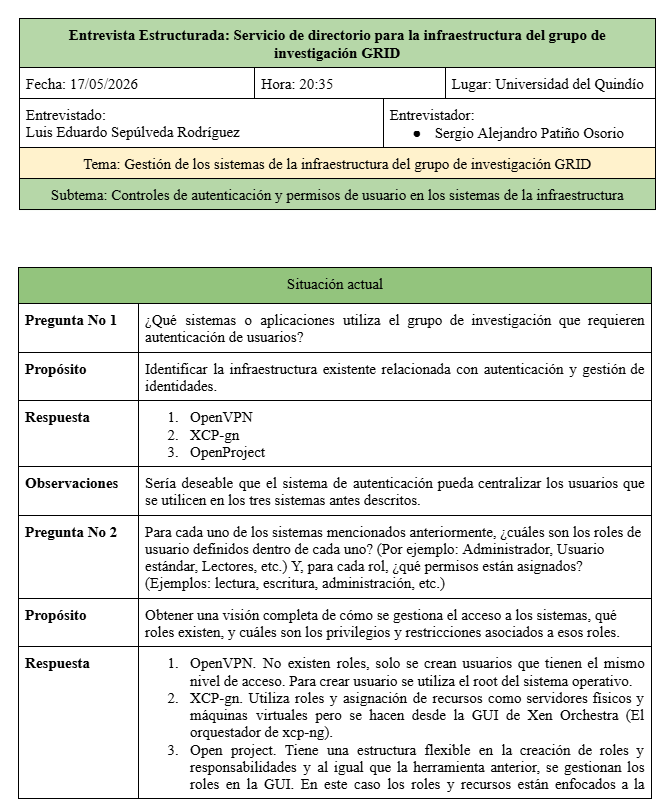
\includegraphics[width=0.7\textwidth]{mainmatter/II-desarrollo-metodologico/caracterizacion-grid/imagenes/vista-general-entrevista.png}
	\caption{Vista general de la entrevista}
	\label{fig:vista-general-entrevista}
\end{figure}

\subsection{Resultados de la entrevista}

A partir de la información recopilada se identificó que la gestión de las cuentas de usuario y el acceso a los diferentes servicios tecnológicos constituían aspectos relevantes para la administración de la infraestructura del \ac{GRID}. La existencia de diferentes servicios con mecanismos propios de autenticación implicaba considerar la necesidad de establecer una gestión más centralizada de las identidades y facilitar la administración de las cuentas.

Asimismo, se identificó la necesidad de establecer mecanismos que permitieran administrar el ciclo de vida de las cuentas de usuario, considerando actividades como su creación, modificación y eliminación. De manera complementaria, se evidenció la importancia de establecer políticas relacionadas con la seguridad de las credenciales y de controlar el acceso a los servicios de acuerdo con los permisos asignados a cada usuario.

Otro aspecto identificado correspondió a la necesidad de fortalecer la capacidad de supervisar los accesos realizados a los servicios y disponer de información que pudiera ser utilizada para fines de seguimiento y auditoría. También se consideró relevante que la solución pudiera integrarse con diferentes servicios tecnológicos y mantener la posibilidad de incorporar nuevos recursos conforme evolucionara la infraestructura del grupo.

La entrevista también permitió identificar expectativas relacionadas con el fortalecimiento de los mecanismos de autenticación y con la recuperación o restablecimiento de las credenciales de los usuarios.

\subsection{Identificación de necesidades, problemas y oportunidades}\label{subsec:identificacion-necesidades}

Como se muestra en la \autoref{tab:npo}, los resultados de la entrevista fueron organizados en términos de \ac{NPO} para relacionar la situación identificada en el \ac{GRID} con los requerimientos que orientarían el desarrollo del proyecto.

\begingroup
\fontsize{8pt}{9pt}\selectfont
\renewcommand{\arraystretch}{1.25}
\setlength{\tabcolsep}{3pt}

\begin{longtable}{|
	>{\centering\arraybackslash}p{0.09\dimexpr\textwidth-6\tabcolsep-5\arrayrulewidth\relax}|
	>{\centering\arraybackslash}p{0.12\dimexpr\textwidth-6\tabcolsep-5\arrayrulewidth\relax}|
	>{\raggedright\arraybackslash}p{0.34\dimexpr\textwidth-6\tabcolsep-5\arrayrulewidth\relax}|
	>{\raggedright\arraybackslash}p{0.45\dimexpr\textwidth-6\tabcolsep-5\arrayrulewidth\relax}|}

	\caption{Necesidades, problemas y oportunidades identificados en la entrevista}
	\label{tab:npo}
	\\
	\hline
	\textbf{ID}                                                                                                     &
	\textbf{Tipo}                                                                                                   &
	\textbf{Necesidad, problema u oportunidad}                                                                      &
	\textbf{Situación identificada}
	\\
	\hline
	\endfirsthead

	\caption[]{Necesidades, problemas y oportunidades identificados en la entrevista (continuación)}
	\\
	\hline
	\textbf{ID}                                                                                                     &
	\textbf{Tipo}                                                                                                   &
	\textbf{Necesidad, problema u oportunidad}                                                                      &
	\textbf{Situación identificada}
	\\
	\hline
	\endhead

	\acs{NPO}-01                                                                                                          &
	Problema                                                                                                        &
	La autenticación de usuarios se encuentra distribuida entre los diferentes sistemas del grupo de investigación. &
	No existe un servicio unificado de autenticación y la gestión de las cuentas se realiza de manera individual en cada herramienta.
	\\
	\hline

	\acs{NPO}-02                                                                                                          &
	Necesidad                                                                                                       &
	Centralizar las cuentas de usuario de OpenVPN, Xen Orchestra y OpenProject.                                     &
	Se identificó la necesidad de centralizar las cuentas utilizadas en los diferentes sistemas.
	\\
	\hline

	\acs{NPO}-03                                                                                                          &
	Problema                                                                                                        &
	La creación, verificación y cierre de cuentas se realiza manualmente.                                           &
	Las actividades relacionadas con la administración de las cuentas se ejecutan de forma manual, situación considerada crítica debido a la necesidad de relacionar la vigencia de las cuentas con situaciones como la terminación de trabajos de grado.
	\\
	\hline

	\acs{NPO}-04                                                                                                          &
	Necesidad                                                                                                       &
	Automatizar el ciclo de vida de las cuentas de usuario.                                                         &
	Se requiere automatizar actividades como la provisión, desprovisión, registro, verificación, revocación y expiración de las credenciales.
	\\
	\hline

	\acs{NPO}-05                                                                                                          &
	Problema                                                                                                        &
	No existe una política estandarizada de contraseñas y acceso.                                                   &
	Se utilizan prácticas no estandarizadas y dependientes de cada usuario para la gestión de contraseñas y acceso.
	\\
	\hline

	\acs{NPO}-06                                                                                                          &
	Necesidad                                                                                                       &
	Establecer políticas coherentes de creación de usuarios y contraseñas.                                          &
	Se requiere establecer un patrón coherente y repetible para la gestión de usuarios y credenciales, considerando buenas prácticas y estándares.
	\\
	\hline

	\acs{NPO}-07                                                                                                          &
	Problema                                                                                                        &
	No se realizan revisiones periódicas de los accesos.                                                            &
	No existen mecanismos establecidos para realizar revisiones periódicas de los accesos de los usuarios.
	\\
	\hline

	\acs{NPO}-08                                                                                                          &
	Necesidad                                                                                                       &
	Implementar mecanismos de control y monitoreo de los accesos.                                                   &
	Se requiere contar con mecanismos para controlar y monitorear los accesos, preferiblemente con capacidad de supervisión en tiempo real.
	\\
	\hline

	\acs{NPO}-09                                                                                                          &
	Problema                                                                                                        &
	No existe un registro centralizado de las actividades relacionadas con usuarios y administradores.              &
	Las actividades asociadas con la gestión de usuarios y administradores no se registran actualmente de manera centralizada.
	\\
	\hline

	\acs{NPO}-10                                                                                                          &
	Necesidad                                                                                                       &
	Contar con trazabilidad y auditoría de las actividades de gestión de accesos.                                   &
	Se requiere registrar las actividades relacionadas con la gestión de accesos para facilitar su seguimiento y posterior auditoría.
	\\
	\hline

	\acs{NPO}-11                                                                                                          &
	Necesidad                                                                                                       &
	Mantener una autorización diferenciada para cada sistema aun cuando las cuentas estén centralizadas.            &
	Se requiere que la centralización de las cuentas no implique que todos los usuarios tengan acceso a los mismos sistemas.
	\\
	\hline

	\acs{NPO}-12                                                                                                          &
	Necesidad                                                                                                       &
	Fortalecer los mecanismos de autenticación mediante políticas de contraseñas, \acs{MFA}, certificados y tokens.       &
	Durante la entrevista se consideró necesario fortalecer la autenticación mediante estos mecanismos, de acuerdo con las necesidades de los servicios.
	\\
	\hline

	\acs{NPO}-13                                                                                                          &
	Necesidad                                                                                                       &
	Establecer mecanismos seguros para la recuperación de contraseñas.                                              &
	Se planteó la posibilidad de utilizar mecanismos de recuperación automática mediante correo electrónico o un segundo factor.
	\\
	\hline

	\acs{NPO}-14                                                                                                          &
	Oportunidad                                                                                                     &
	Preparar la infraestructura de autenticación para incorporar activos de información de mayor valor.             &
	Aunque el impacto actual de un acceso no autorizado se considera medio, se prevé la incorporación futura de activos de mayor valor.
	\\
	\hline
\end{longtable}
\endgroup


La identificación de estos aspectos permitió establecer una base para la definición de los requerimientos funcionales y no funcionales considerados en el proyecto. De esta manera, los hallazgos obtenidos durante la entrevista fueron utilizados como insumo para orientar la identificación de una tecnología de servicio de directorio y posteriormente evaluar su capacidad para responder a las necesidades planteadas en el contexto del \ac{GRID}.
